\chapter{Metod}

Den metodik som tillämpats vid beräkning av olika energiflöden bygger på det teoretiska underlag som presenterats i föregående kapitel. Byggnaden kommer här delas upp i de två beståndsdelarna grunden – som påverkas av vädret via marken som värmebuffert – och byggnadsskalet – med väggar, tak och fönster vars ytor direkt påverkas av vädret. Dessutom tillkommer solinstrålningen genom fönster och ofrivillig ventilation på grund av vind, vilka betraktas helt fristående.

Vi börjar med de analytiska beräkningar som beskriver solinstrålningen och går sedan direkt in på att beskriva hur ett statiskt värmeflöde genom en vägg kan beräknas. Vidare beskrivs hur finita elementmetoden har används för att behandla statiska luftflöden, som här nyttjats för att beräkna luftflödet längs väggen när det blåser.

Slutligen finns ett avsnitt som beskriver hur man med hjälp av programmet Comsol Multiphysics kan beräkna påverkan på fastigheten från ofrivillig ventilation, det vill säga hur mycket energi som försvinner genom vind som penetrerar huset. 

\subsubsection{Solstrålning genom fönster}

För att beräkna den totala effekt solstrålning tillför byggnaden behövs fönstrenas vinkelberoende g-värden (presenterat i avsnitt \ref{gvalue}). 

För att beräkna g-värdet ur \eqref{eq:radiationwindowstheory:gvalue} behöver parametern $z = \theta/90$ beräknas, där $\theta$ är vinkeln mellan solstrålingens riktning och fönstrets normal. Detta kan göras genom att utgå från aktuellt datum och tid på dygnet.

En metod för att räkna ut solens position presenteras i \cite{walraven78} och en Matlabfunktion baserad på samma artikel kan ses i appendix. % Hänvisa till kod

Om azimuthala och altitudinella vinklarna ($\beta$ respektive $\alpha$) relativt ett väderstreck respektive horisonten tillhandahålls beräknas infallsvinkeln mot glaset, $\theta$, på följande vis:

\begin{equation} 
\theta = \frac{360}{2\pi}\arctan{\left( \sqrt{\tan^2{\left(\alpha\right)}
+ \tan^2{\left(\beta - \gamma \right)}} \right)}
\end{equation}

där $\gamma$ är vinkeln mellan fönstrets normal och väderstrecket mot vilken azimuthala vinkeln anges. Notera att alla vinklar utom $\theta$ anges i radianer.

Med dessa samband tillgängliga kan ett Matlabprogram för beräkning av effektflödet på grund av solstrålning genom fönster skapas, och ett exempel kan ses i appendix. % Hänvisa till appendix.

% Behöver: longitud, latitud, vinkeln relativt väderstreck, fönsters area, g-värde

\subsubsection{Inverkan av skuggor, gardiner och dylikt}

% Beräkna för vilka vinklar skuggor faller över fönstren

% Gardiner, persienner och interiör förändrar situationen, kolla källan nedan
\begin{comment}
Simmler & Binder
Experimental and numerical determination of the total solar energy transmittance of glazing with venetian blind shading
\end{comment}

% Be Särnöe om specifikationer:
% - I vilket väderstreck är normalen riktad?
% - Vilket g-värde har fönstren?

\begin{comment}
I diskussion:
- Hur kan man koppla detta till värmesystemet?
	- Registrera intensitet, tid på dygnet och datum
	- Beräkna ungefärlig tillförd effekt
	- Kompensera genom att säga till värmesystemet att minska/stänga inflödet
- Blir det lättare att helt enkelt mäta temperaturen i rummet och gå utifrån det? Vad är mer kostnadseffektivt?
\end{comment}

\section{Finita element av värmeledningsekvationen}
\label{sec:femheat}
I detta avsnitt behandlas finita elementlösningen av värmeledningsekvationen.
Det är från avsnitt \ref{sec:heatconduction} givet att differentialekvationen
enligt ekvation \eqref{eq:femheateq} beskriver värmeflöde i ett material.

\begin{equation}
\label{eq:femheateq}
c_p\rho\frac{\partial T}{\partial t} = \nabla\cdot(k\nabla T)
\end{equation}

\noindent
För att finna en lösning integreras värmeledningsekvationen
multiplicerat med en $L^2$ integrabel testfunktion $\phi(\mathbf{r})$ över hela
definitionsmängden $\Omega$ vars rand benämns $\Gamma$.
Detta kan ses i ekvation \eqref{eq:femheatweak}.
Nu söks en funktion $T(\mathbf{r},t)$ som satisfierar nyss nämnda uttryck för
alla $L^2$ integrabla testfunktioner $\phi(\mathbf{r})$.

\begin{equation}
\label{eq:femheatweak}
\int_\Omega \left(c_p\rho\frac{\partial T}{\partial t} -
\nabla\cdot(k\nabla T)\right)\phi(\mathbf{r})d\Omega = 0
\end{equation}

\noindent
För att förenkla fortsatta beräkningar behövers det genomföras några
omskrivningar av uttrycket. Divergensteoremet används först för att 
eliminera divergensen i värmeledningsekvationens högerled. Detta ger då
ekvation \eqref{eq:femheatweakfull}. Här är $\mathbf{n}$ normalen till randen.

\begin{equation}
\label{eq:femheatweakfull}
\int_\Omega c_p\rho\frac{\partial T}{\partial t}\phi(\mathbf{r}) +
k\nabla T\nabla\phi(\mathbf{r}) d\Omega =
\int_\Gamma k\mathbf{n}\cdot\nabla Td\Gamma
\end{equation}

\noindent
Härnäst skall galerkinformuleringen skissas. Detta genomförs
genom att temperaturen $T$ samt tidsderivatan av temperaturen $\dot{T}$
enligt ekvationerna \eqref{eq:femheatt} och \eqref{eq:femheattdot}.

\begin{align}
\label{eq:femheatt}
T(\mathbf{r}) & \approx \sum_n T_n\phi(\mathbf{r}) \\
\label{eq:femheattdot}
\dot{T}(\mathbf{r}) & \approx \sum_n \dot{T}_n\phi(\mathbf{r})
\end{align}

\noindent
Ansatsen ovan stoppas härnäst in i den svaga formuleringen i ekvation
\eqref{eq:femheatweakfull} vilket ger ekvation \eqref{eq:femheatgalerkin}.
För att kunna lösa problemet för definitionsmängder som består av olika
homogena material väljs testfunktionen $\phi$ så att den försvinner vid
alla andra material än ett och värmeledningskonstanten kan då benämnas $k_n$.
Ekvationssystemet kan sedan skrivas i matrisform vilket kan ses i ekvation
\eqref{eq:femheatmatrix}. Här är $M$ massmatrisen, $A$ är stelhetsmatrisen och
$f$ är belastningsvektorn.

\begin{align}
\label{eq:femheatgalerkin}
\sum_n \dot{T}_n \int_\Omega c_p\rho\phi_i(\mathbf{r})
\phi_n(\mathbf{r})d\Omega
& + \sum_n T_n \int_\Omega k_n \nabla\phi_n(\mathbf{r})\nabla\phi_n(\mathbf{r})
d\Omega \\
&= \int_\Gamma k_i\phi_i\mathbf{n}\cdot\nabla Td\Gamma \Leftrightarrow
\nonumber
\end{align}

\begin{equation}
\label{eq:femheatmatrix}
M\dot{T} + AT = f \Rightarrow
\end{equation}

\begin{equation}
\label{eq:femheatmatrix2}
\dot{T} + M^{-1}AT = M^{-1}f
\end{equation}

\noindent
Som kan ses så är ovanstående uttryck ett system av kopplade ordinära
differentialekvationer vars lösning är trivial med hjälp av egenvärdesuppdelning.
Vektorerna $\{v\}^n_{i=1}$ definieras som egenvektorerna av
$M^{-1}A$ och $\lambda_i$ definieras som egenvärdena till samma matris.
Systemets homogena lösning kan då skrivas som ekvation
\eqref{eq:femheathom}.\cite{lay06}

\begin{equation}
\label{eq:femheathom}
T_h(t) = \sum_n = c_nv_ne^{-\lambda_nt}
\end{equation}

\noindent
Då ekvationen är inhomogen så återstår det att lösa systemets
partikulärlösning. Då inhomogeniteten är konstant så kan lämpligen
en konstant ansättas som partikulärlösning. Detta ger att
$T_p(t) = D$. Insättning i differentialekvationen ger
ekvation \eqref{eq:femheatinstopp} vilket gör att vi kan bestämma
$D$ genom ekvation \eqref{eq:femheatinstopp2}.

\begin{align}
\label{eq:femheatinstopp}
M^{-1}AD &= M^{-1}b \Rightarrow\\
\label{eq:femheatinstopp2}
D &= A^{-1}b
\end{align}

\noindent
Nu kan den fullständiga lösningen skissas som $T = T_h + T_p$ och om
tiden sätts till noll så kan konstanterna $c_n$ bestämmas genom
att $T$ sätts till problemets begynnelsevärden. För ett problem som
saknar tidsberoende eller som har nått en jämviktspunkt måste
tiden vara oändlig och de termer som innehar exponenter blir noll.
Detta innebär att partikulärlösningen $T_p$ är den tidsoberoende lösningen
till problemet. Detta kan enkelt verifieras genom att sätta $\dot{T} = 0$.
Problemet som återstår är då $AT = b$ vars lösning är $T_p$.

\section{Värmeflöde i vägg}

För att beskriva ett värmeflöde används ekvationerna Fouriers värmeekvation
\eqref{eq:conduction:fourier} och värmeledningsekvationen 
\eqref{eq:conduction:heateq}. 
I dessa är
$k$ värmeledningsförmågan\\i $\mbox{W}\mbox{m}^{-2}\mbox{K}^{-1}$ och
$\alpha$ är termisk diffusivitet i $\mbox{m}^2\mbox{s}^{-1}$. \cite{physicshandbook}

Vid statiskt värmeflöde kommer temperaturderivatan med avseende på tiden att vara noll.
Detta innebär att värmeledningsekvationen övergår i Laplaces ekvation
$\Delta{}T = 0$. I en dimension blir detta $d^2T/dx^2 = 0$ vilket innebär
att lösningen blir ett polynom av första ordningen.  

\begin{equation}
%\label{eq:staticwallmethod:fourier}
q_x = -k \frac{dT}{dx}
\tag{\ref{eq:conduction:fourier}}
\end{equation}

\begin{equation}
%\label{eq:staticwallmethod:heat}
\frac{\partial T}{\partial t} = \alpha \Delta T
\tag{\ref{eq:conduction:heateq}}
\end{equation}

\noindent
Vi vill nu beskriva det statiska värmeflödet genom en vägg som består
av flera olika material. De enda värmekällorna som påverkar väggen
är en isoterm $T = T_H$ på ena sidan av väggen
samt en isoterm $T = T_L$ på andra sidan av väggen.

För att göra beräkningarna enklare
ser vi väggen som en oändligt stor skiva. Detta innebär att vi kan räkna
på ekvationen i en dimension. Med hjälp av det härledda sambandet i avsnitt \ref{sec:heatconduction} kan ett ekvationssystem bildas.

\begin{equation}
\label{eq:staticwalltheory:rodmatrix}
\begin{pmatrix}
Q \\
-Q
\end{pmatrix} = 
\frac{k}{L}\begin{pmatrix}
1 & -1 \\
-1 & 1
\end{pmatrix}
\begin{pmatrix}
T_1 \\
T_2
\end{pmatrix}
\end{equation}

\noindent
Vi kan nu teckna dessa ekvationssystem för alla delar av väggen, som skrivs som 
en matris och sedan fylla ut matriserna med nollelement för att slutligen bilda 
en linjärkomination.
Då linjärkombinationen bildas kommer energiflödena i mitten av väggen att
vara noll. Detta överensstämmer väl med att vi har en statisk energifördelning
utan interna värmekällor.
Slutligen får vi ett ekvationsystem enligt ekvation
\eqref{eq:staticwallmethod:full} som enkelt kan lösas.
Matrisen $A$ är linjärkombinationen av nollutfyllda versioner av matrisen i ekvation
\eqref{eq:staticwalltheory:rodmatrix} enligt ekvation
\eqref{eq:staticwallmethod:example}.

\begin{equation}
\label{eq:staticwallmethod:example}
A = \frac{k_1}{L_1}
\begin{pmatrix}
1 & -1 & 0 &  \dots \\
-1 & 1 & 0 &   \\
0 & 0 & 0 &  \\
\vdots & & & \ddots
\end{pmatrix}
+
\frac{k_2}{L_2}
\begin{pmatrix}
0 & 0 & 0 & 0 & \dots \\
0 & 1 & -1 & 0 &  \\
0 & -1 & 1 & 0 & \\
0 & 0 & 0 & 0 & \\
\vdots & & & & \ddots
\end{pmatrix} + \dots
\end{equation}

\begin{equation}
\label{eq:staticwallmethod:full}
\begin{pmatrix}
Q\\0\\...\\0\\-Q
\end{pmatrix} = A
\begin{pmatrix}
T_H\\T_1\\...\\T_{n-1}\\T_L
\end{pmatrix}
\end{equation}

Här gör vi en jämförelse mellan en oisolerad, 50 cm tjock tegelvägg, motsvarande den som finns på fastighetens södersida, och en 50 cm tjock tegelvägg med 10 cm isolering, motsvarande den som finns på fastighetens norrsida.

\section{Finita element av värmeledningsekvationen}
\label{sec:femheat}
I detta avsnitt behandlas finita elementlösningen av värmeledningsekvationen.
Det är från avsnitt \ref{sec:heatconduction} givet att differentialekvationen
enligt ekvation \eqref{eq:femheateq} beskriver värmeflöde i ett material.

\begin{equation}
\label{eq:femheateq}
c_p\rho\frac{\partial T}{\partial t} = \nabla\cdot(k\nabla T)
\end{equation}

\noindent
För att finna en lösning integreras värmeledningsekvationen
multiplicerat med en $L^2$ integrabel testfunktion $\phi(\mathbf{r})$ över hela
definitionsmängden $\Omega$ vars rand benämns $\Gamma$.
Detta kan ses i ekvation \eqref{eq:femheatweak}.
Nu söks en funktion $T(\mathbf{r},t)$ som satisfierar nyss nämnda uttryck för
alla $L^2$ integrabla testfunktioner $\phi(\mathbf{r})$.

\begin{equation}
\label{eq:femheatweak}
\int_\Omega \left(c_p\rho\frac{\partial T}{\partial t} -
\nabla\cdot(k\nabla T)\right)\phi(\mathbf{r})d\Omega = 0
\end{equation}

\noindent
För att förenkla fortsatta beräkningar behövers det genomföras några
omskrivningar av uttrycket. Divergensteoremet används först för att 
eliminera divergensen i värmeledningsekvationens högerled. Detta ger då
ekvation \eqref{eq:femheatweakfull}. Här är $\mathbf{n}$ normalen till randen.

\begin{equation}
\label{eq:femheatweakfull}
\int_\Omega c_p\rho\frac{\partial T}{\partial t}\phi(\mathbf{r}) +
k\nabla T\nabla\phi(\mathbf{r}) d\Omega =
\int_\Gamma k\mathbf{n}\cdot\nabla Td\Gamma
\end{equation}

\noindent
Härnäst skall galerkinformuleringen skissas. Detta genomförs
genom att temperaturen $T$ samt tidsderivatan av temperaturen $\dot{T}$
enligt ekvationerna \eqref{eq:femheatt} och \eqref{eq:femheattdot}.

\begin{align}
\label{eq:femheatt}
T(\mathbf{r}) & \approx \sum_n T_n\phi(\mathbf{r}) \\
\label{eq:femheattdot}
\dot{T}(\mathbf{r}) & \approx \sum_n \dot{T}_n\phi(\mathbf{r})
\end{align}

\noindent
Ansatsen ovan stoppas härnäst in i den svaga formuleringen i ekvation
\eqref{eq:femheatweakfull} vilket ger ekvation \eqref{eq:femheatgalerkin}.
För att kunna lösa problemet för definitionsmängder som består av olika
homogena material väljs testfunktionen $\phi$ så att den försvinner vid
alla andra material än ett och värmeledningskonstanten kan då benämnas $k_n$.
Ekvationssystemet kan sedan skrivas i matrisform vilket kan ses i ekvation
\eqref{eq:femheatmatrix}. Här är $M$ massmatrisen, $A$ är stelhetsmatrisen och
$f$ är belastningsvektorn.

\begin{align}
\label{eq:femheatgalerkin}
\sum_n \dot{T}_n \int_\Omega c_p\rho\phi_i(\mathbf{r})
\phi_n(\mathbf{r})d\Omega
& + \sum_n T_n \int_\Omega k_n \nabla\phi_n(\mathbf{r})\nabla\phi_n(\mathbf{r})
d\Omega \\
&= \int_\Gamma k_i\phi_i\mathbf{n}\cdot\nabla Td\Gamma \Leftrightarrow
\nonumber
\end{align}

\begin{equation}
\label{eq:femheatmatrix}
M\dot{T} + AT = f \Rightarrow
\end{equation}

\begin{equation}
\label{eq:femheatmatrix2}
\dot{T} + M^{-1}AT = M^{-1}f
\end{equation}

\noindent
Som kan ses så är ovanstående uttryck ett system av kopplade ordinära
differentialekvationer vars lösning är trivial med hjälp av egenvärdesuppdelning.
Vektorerna $\{v\}^n_{i=1}$ definieras som egenvektorerna av
$M^{-1}A$ och $\lambda_i$ definieras som egenvärdena till samma matris.
Systemets homogena lösning kan då skrivas som ekvation
\eqref{eq:femheathom}.\cite{lay06}

\begin{equation}
\label{eq:femheathom}
T_h(t) = \sum_n = c_nv_ne^{-\lambda_nt}
\end{equation}

\noindent
Då ekvationen är inhomogen så återstår det att lösa systemets
partikulärlösning. Då inhomogeniteten är konstant så kan lämpligen
en konstant ansättas som partikulärlösning. Detta ger att
$T_p(t) = D$. Insättning i differentialekvationen ger
ekvation \eqref{eq:femheatinstopp} vilket gör att vi kan bestämma
$D$ genom ekvation \eqref{eq:femheatinstopp2}.

\begin{align}
\label{eq:femheatinstopp}
M^{-1}AD &= M^{-1}b \Rightarrow\\
\label{eq:femheatinstopp2}
D &= A^{-1}b
\end{align}

\noindent
Nu kan den fullständiga lösningen skissas som $T = T_h + T_p$ och om
tiden sätts till noll så kan konstanterna $c_n$ bestämmas genom
att $T$ sätts till problemets begynnelsevärden. För ett problem som
saknar tidsberoende eller som har nått en jämviktspunkt måste
tiden vara oändlig och de termer som innehar exponenter blir noll.
Detta innebär att partikulärlösningen $T_p$ är den tidsoberoende lösningen
till problemet. Detta kan enkelt verifieras genom att sätta $\dot{T} = 0$.
Problemet som återstår är då $AT = b$ vars lösning är $T_p$.


\section{Värmeflöde genom grunden}

För att räkna på energin som flödar genom grunden är det nödvämdigt att räkna
transient. Detta då berget tar åt sig värme väldigt långsamt. I praktien innebär detta att ett statiskt jämviktsläge aldrig uppnås.

Problemet är behandlat med finita elementmetoden av värmeledningsekvationen.
Geometrin av problemet och trianguleringen kan ses i figur \ref{fig:foundation:tri}.
Randvärdena som är satt är att alla rander som går från berg till berg är adiabatiska.
Detta kommer inte stämma i praktiken om inte definitionsmängden sätts till oändligt
stor. För lösning av detta problem kan det dock ses som en tillräckligt god
approximation eftersom definitionsmängden är stor och temperaturen inte varierar så mycket
från förväntat värde.

Vid randerna mot grunden ligger ett neumannvillkor som säger att energiflödet är produkten
av temperaturdifferansen mellan temperaturen på randen och inomhustemperaturen på $\unit[20]{^\circ C}$.
Grundens U-värde har här satts till $U = 0,7/0,45 \approx \unit[1,556]{ Wm^{-2}K^{-1}}$. Detta värde är
baserat på att det ligger $\unit[0,25]{m}$ betong mellan källaren och grunden och att det ligger ytterligare $\unit[0,2]{m}$
betong mellan uppvärmda utrymmen och källaren. Vidare antas att det föreligger god omrörning i de båda
luftskikten vilket gör att de har $R=0$. Detta antagande är dock inte helt giltigt vilket leder till att kyleffekten
uppskattas vara något för hög.
Vid randerna till luft är konvektionsparametern satt
till $h = \unit[15,5]{Wm^{-2}K^{-1}}$. Detta är en siffra som motsvarar
en vindhastighet på ungefär $v = \unit[2]{ms^{-1}}$. Utomhustemperaturen har valts
som en minstakvadratanpassad trigonetrisk funktion av
medeltemperaturen de senaste tjugo åren vilket kan ses i figur
\ref{fig:foundation:meantemperature}. Anpassningen gör att
differentialekvationerna av galerkinformuleringen kan lösas analytiskt
för alla tider istället för att systemet ska behöva lösas semidiskret.
Detta minskade exekveringstiden dramatiskt vilket gav möjlighet att använda en
mycket finare triangulering. Dessutom kan alla termer i lösningen
som går mot noll då tiden går mot oändligeheten sättas till noll. Detta innebär
att få lösningar når ett transient jämviktsläge som liknar det jämviktsläge vi har i praktiken.
Initialvärdena kommer således inte ha någon betydelse och dessa kan då väljas
godtyckligt. 
För att uppnå detta resultat med semidiskret MOL behövs väldigt många itereringar för att
nå konvergens. Den resulterande koden kan ses i bilaga \ref{app:femfoundation}.

\begin{figure}
\centering
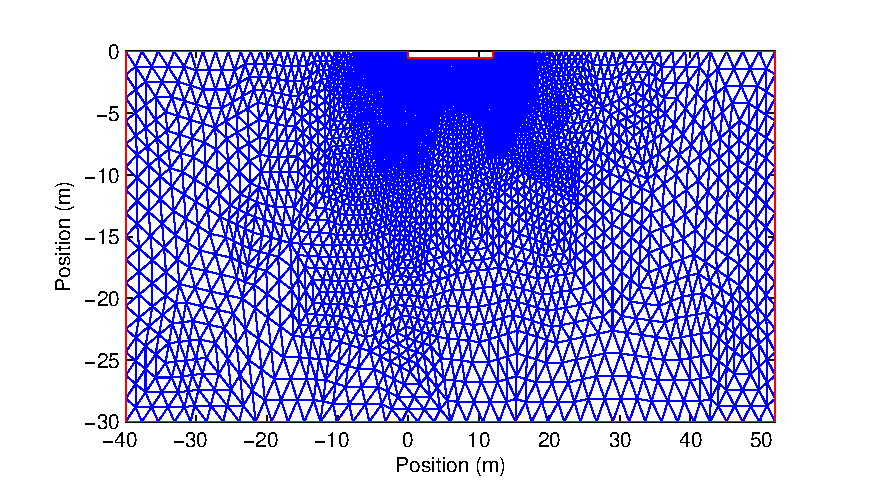
\includegraphics{images/trifoundation.eps}
\caption{Definitionsmängd och triangulering berget under grunden.}
\label{fig:foundation:tri}
\end{figure}


\begin{figure}
\centering
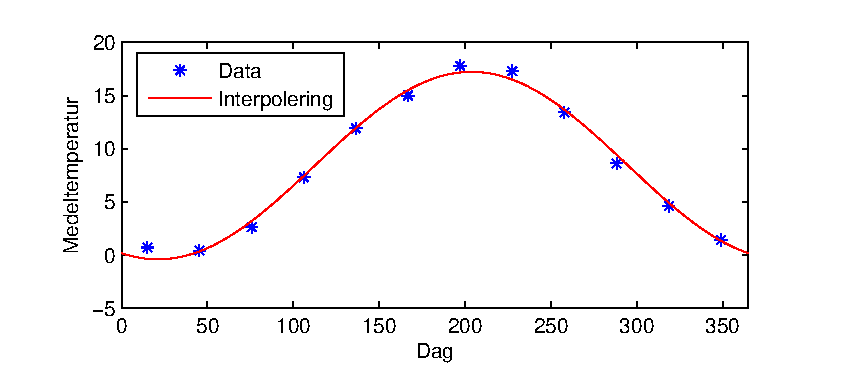
\includegraphics{images/meantemperature.eps}
\caption{
Medeltemperaturen för Göteborg de senaste 20 åren. Punkterna är data tagna från Miljöförvaltningen och linjen är minstakvadratanpassningen som senare använts för att beräkna energiflöden.}
\label{fig:foundation:meantemperature}
\end{figure}

%Miljöförvaltningen
%http://www4.goteborg.se/prod%5Csk%5Cstatistik%5CstatistikR5.nsf/0/3F002A395ED39AC8C1256D3B00393D0E/$File/3.01.pdf

\subsection{Finita element av inkompressibel fluid}

För att lösa Navier-Stokes ekvationer kan lämpligen en datormodell användas.
Här består denna modell av ett system uppsatt med Galerkins metod.
I denna lösning så begränsar vi dock oss till att enbart behandla statiska flöden
vilket genomförs genom att sätta alla tidsderivator till noll.

För att hantera trycket i \eqref{eq:convection:continuity}-\eqref{eq:convection:energy} används den tidigare nämnda Boussinesq approximation
samt penalty metoden för att göra hastighetsvektorn källfri och uppfylla
kontinuitetsekvationen. Det finns således inget direkt behov av att räkna ut trycket.
Vid användning av många sorters elementtyper som inte uppfyller Babuska-Brezzikriteriet
är detta dessutom nödvändigt då det annars kan bildas oönskade trycknoder. 
En annan möjlighet är att välja divergensfria element. \cite{babuska1973}\cite{segal2011}

Genom penaltymetoden beskrives här trycket som $p$ enligt ekvation
\eqref{eq:femconvection:penalty}. Här är $p_s$ någon form av idealt statiskt
tryck som är önskat. Detta tryck följer Boussinesq approximation. Med dessa
idealiseringar kan differentialekvationerna sättas upp igen. \cite{heinrich88}\cite{taylor79}
Som kan ses så leder den godtyckliga penaltyparametern $\lambda$ till att justera trycket
om hastighetsfältets divergens ej är identiskt noll. I viss litteratur anges 
det att penaltyparametern skall vara i storleksordningen $10^7$ men att den
är väldigt applikationsberoende. En för liten vald penaltyparameter leder till att
trycket inte elimineras. Andra problem uppstår vid en för stor parameter. Ekvationssystemet
kan bli svårlöst och få stabilitetsproblem när parametern blir
för stor i jämförelse med de andra delarna i differentialekvationen.\cite{reddy93}\cite{roy05}\cite{basak04}\cite{segal2011}

\begin{equation}
\label{eq:femconvection:penalty}
p = p_s - \lambda\nabla\cdot\mathbf{v}
\end{equation}

\noindent
Fortsatt skall trycket deriveras med avseende på de rumsliga variablerna vilket möjliggör
att eliminera trycket från differentialekvationerna. Dessa deriveringar kan ses i ekvation
\eqref{eq:femconvection:partx} samt \eqref{eq:femconvection:partz}. Notera att det statiska trycket
$p_s$ ej beror på $x$ vilket resulterar i att derivatan är noll.

\begin{equation}
\label{eq:femconvection:partx}
\frac{\partial p}{\partial x} = \frac{\partial p_s}{\partial x} -
\frac{\partial}{\partial x} \lambda\nabla\cdot\mathbf{v} = -
\frac{\partial}{\partial x} \lambda\nabla\cdot\mathbf{v}
\end{equation}

\begin{equation}
\label{eq:femconvection:partz}
\frac{\partial p}{\partial z} = \frac{\partial p_s}{\partial z} -
\frac{\partial}{\partial z} \lambda\nabla\cdot\mathbf{v} =
-g\rho_0 - \frac{\partial}{\partial z} \lambda\nabla\cdot\mathbf{v}
\end{equation}

\noindent
Detta förs in i momentekvationerna vilket ger ekvationerna \eqref{eq:femconvection:u} -
\eqref{eq:femconvection:T}. Här är det ekvationssystem som syftar att lösas.

\begin{equation}
\label{eq:femconvection:u}
\mathbf{v}\cdot\nabla u =
\frac{\lambda}{\rho_0}\nabla\cdot\mathbf{v} +
\nu\Delta u
\end{equation}

\begin{equation}
\label{eq:femconvection:w}
\mathbf{v}\cdot\nabla w =
\frac{\lambda}{\rho_0}\nabla\cdot\mathbf{v} + \nu\Delta w +g\beta(T-T_0)
\end{equation}

\begin{equation}
\label{eq:femconvection:T}
\mathbf{v}\cdot\nabla T = \alpha\Delta T
\end{equation}

\subsubsection{Svag formulering}

En finita elementlösning med Galerkins metod kräver att problemet reduceras till
ett ekvivalent variationsproblem. Här söks $T\in\Phi$, $u\in\Phi$ och
$w\in\Phi$ som uppfyller ekvation \eqref{eq:femconvection:variation}. Här
betecknar brackets skalärprodukt, $\mathbf{L}$ är differentialoperatorn
som betecknar systemet av differentialekvationer som $\mathbf{L}(T,u,w) = 0$.
$\Phi$ är rummet av alla testfunktioner $\phi$ som är kontinuerliga i
definitionsmängden $\Omega$ samt vars derivator är bitvis kontinuerliga på randen
$/Gamma$. De måste även vara $L^2$ integrabla.

\begin{equation*}
\label{eq:femconvection:variation}
\langle \mathbf{L}(T,u,w), \phi \rangle = 0\mbox{,  } \forall \phi \in \Phi
\end{equation*}


\section{Studie av konvektionsparametern}

Finita element har använts även för att studera konvektionsparametern. Hastigheterna har alla
sats till noll på randerna med $h=\unit[6,19]{W~m^{-2}~K^{-1}}$ vilket motsvarar en helt vindstilla dag.
Husets tak är adiabadiskt
och problemet är studerat under en natt i jämviktsläge, det vill säga en evig natt, med
$T_\text{ref} = \unit[0]{^\circ C}$ som referenstemperatur och $T_\text{inne} = \unit[20]{^\circ C}$ inomhus.
Väggens U-värde är satt till $U = \unit[1,19]{W~m^{-2}~K^{-1}}$ vilket motsvarar den oisolerade söderväggen på fastigheten på Walleriusgatan. Penaltyparametern är satt till $\lambda = 10^7$ \emph{\color{Enhet på penaltyparametern}}.

\begin{figure}
\centering
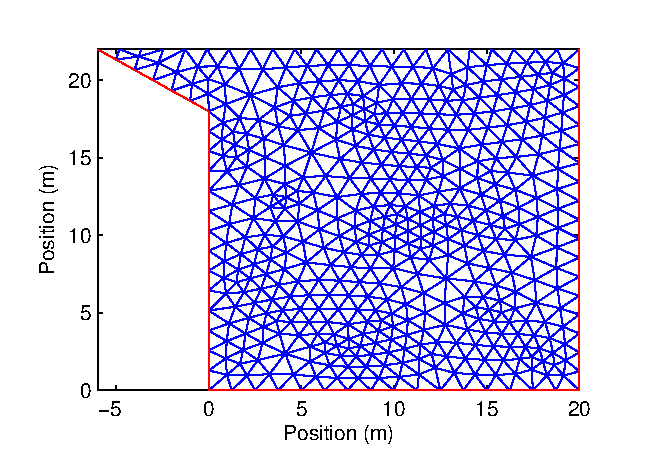
\includegraphics{images/triconvec.eps}
\caption{Definitionsmängd samt triangulering av problemuppställningen för studie av konvektion.}
\end{figure}

Svartkroppsstrålningen approximeras med första ordningens taylorutveckling och
för varje steg löses det slutgiltiga ekvationssystemet med den
modifierade Newton-Raphsons metod. När systemet har lösts beräknas
medeltemperaturen på väggen. Denna används sedan som gissning och utvecklingspunkt
för ovan nämnda taylorutveckling. Denna process upprepas tills medeltemperaturen
ligger tillräckligt nära gissningen. Således genomförs en rad newtonsteg
för att bestämma strålningseffekten från fastigheten genom svartkroppsstrålning.

Sist beräknas konvektionsparametern då mängden energi som transporteras
genom luften är känd. I jämvikt gäller

\begin{equation}
\label{eq:convectionmethod:balance}
Q_\text{vägg} + Q_\text{svartkropp} = Q_\text{konvektion}
\end{equation}

Här är $Q_\text{vägg}$ energin som flödar genom väggen, $Q_\text{svartkropp}$ är energin från
svartkroppsstrålning och $Q_\text{konvektion}$ är då energin som transporteras med konvektion
för att jämvikt skall uppstå.

Medeltemperaturen $\bar{T}$ på väggen och referenstemperaturen $T_\infty$ är kända
vilket ger att h-värdet kan beräknas enligt

\begin{align}
Q_\text{konvektion} &= h(\bar{T}-T_\infty) \Rightarrow \nonumber \\
h &= \frac{Q_\text{vägg} + Q_\text{svartkropp}}{\bar{T}-T_\infty}
\end{align}


\begin{figure}[hpbt]
\centering
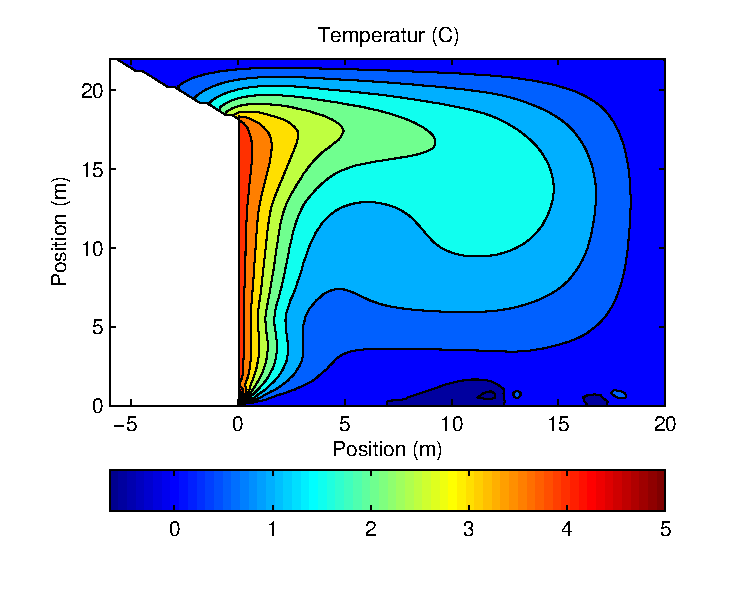
\includegraphics[width=10cm]{images/convectemperature.eps}
\caption{\label{fig:temp_dist}Temperaturfördelningen i $^\circ\mbox{C}$ utanför en vägg, beräknad med finita element av penalty-metoden. Inomhus\-tempertur $\unit[20]{^\circ C}$, utomhustemperatur $\unit[0]{^\circ C}$.}
\end{figure}

% RESULTAT                                                                                                                                    
Denna metod har slutligen verifierats. Som kan ses i figuren~\ref{fig:temp_dist} är luften närmast väggen upp till fem grader 
högre än omgivningen. När det blåser försvinner den här temperaturskillnaden. Detta
visar tydligt hur viktigt det är att inte bara reglera efter utomhustemperaturen.
Här finns dock anomala temperaturer vid nedre randen. Detta tyder på problem med
metodiken.
%%%%%%%%%%%%%%%%%%%%%%%%%%%%%%%%%%%%%%%%%%%%                                                                                                  
Även hastighetsfältet för temperaturens flöde då det är vindstilla har beräknats med finita element metoden
applicerad på penalty-metoden. Detta kan ses i figur~\ref{fig:velocityfield} där också
beloppet av hastighetsfältet visas och det kan noteras att hastigheterna orimligt små.

\begin{figure}[hpbt]
\begin{center}
\subfloat[Hastighetsfält]{
\raisebox{1.2cm}
	{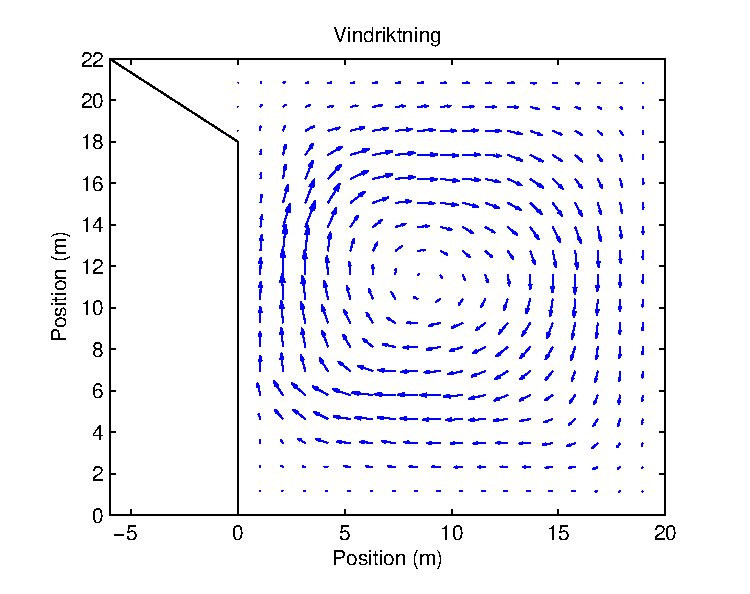
\includegraphics[height=4.9cm]{images/convecquiver.eps}
}}
\subfloat[Beloppet av hastigheten]{
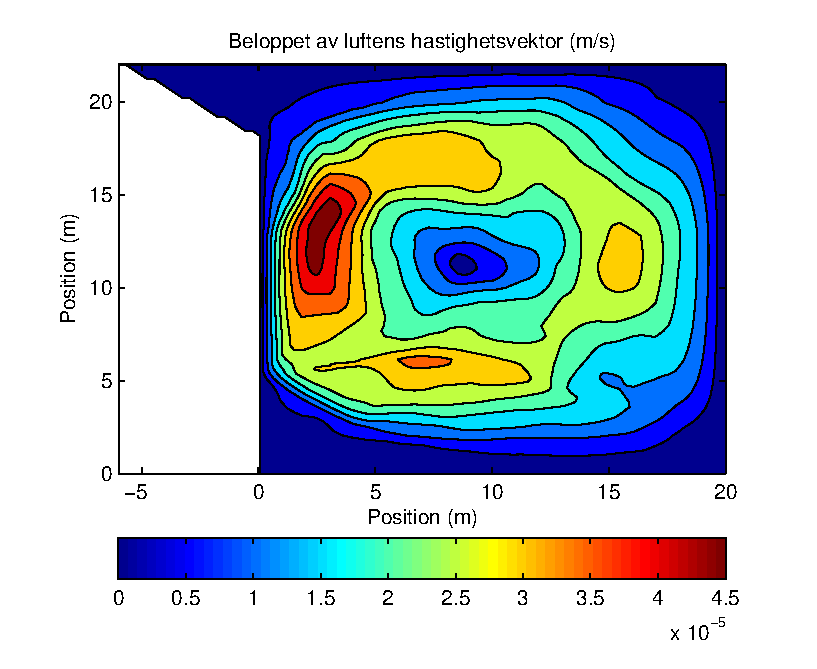
\includegraphics[height=6.2cm]{images/convecspeed.eps}
}
\caption{\label{fig:velocityfield} Hur luften vid husväggen flödar vid en temperaturskillnad.}
\end{center}
\end{figure}


Då sedan konvektionsparametern beräknas utifrån detta blir den väldigt liten,
se figur~\ref{fig:konv_param}. Tyvärr verkade det inte som att metodiken som användes
för att framställa ovanstående data fungerade tillräckligt bra för att med någon
noggrannhet studera fenomenet konvektion. Vi menar dock att formen på hastighetsflödet intill marken och väggen
kan anses vara av rätt karaktär och visar på hur luften rör sig vid husväggen. Randerna mot
luft kan påverka då det inte var tillåtet för luften att passera där, vilket också kan vara en felkälla till den absurt låga konvektionsparametern.

\begin{figure}[hpbt]
\centering
\subfloat[\label{fig:h_reftemp}Konvektions\-koefficienten h mot referens\-temperaturen.]{
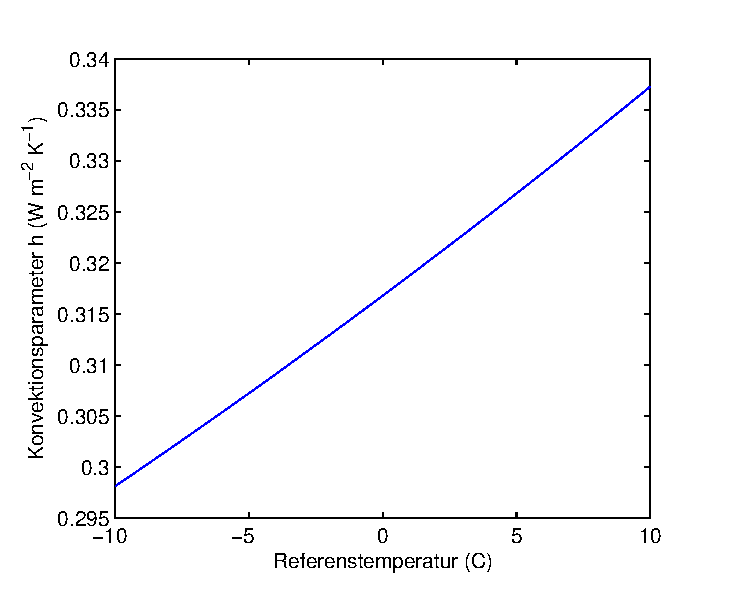
\includegraphics[scale=0.5]{images/convech.eps}
}
\subfloat[\label{fig:h_penalty}Konvektions\-koefficienten h mot penalty\-parametern.]{
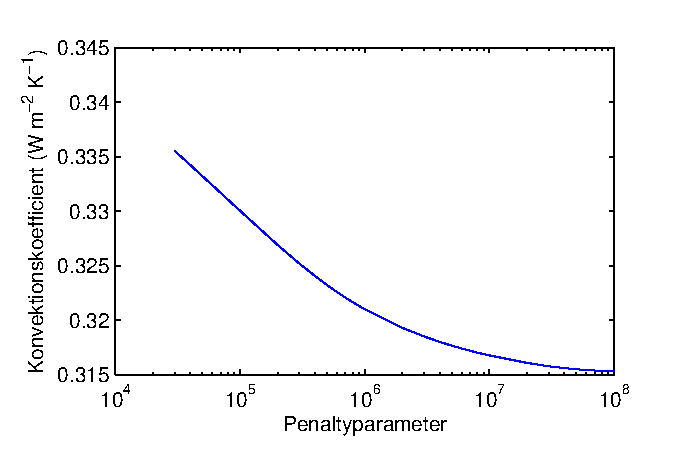
\includegraphics[scale=0.5]{images/convecpenalty.eps}
}\vspace{1cm}

\subfloat[\label{fig:h_volexp}Konvektions\-koefficienten h mot den volymetriska expansions\-koefficienten.]{
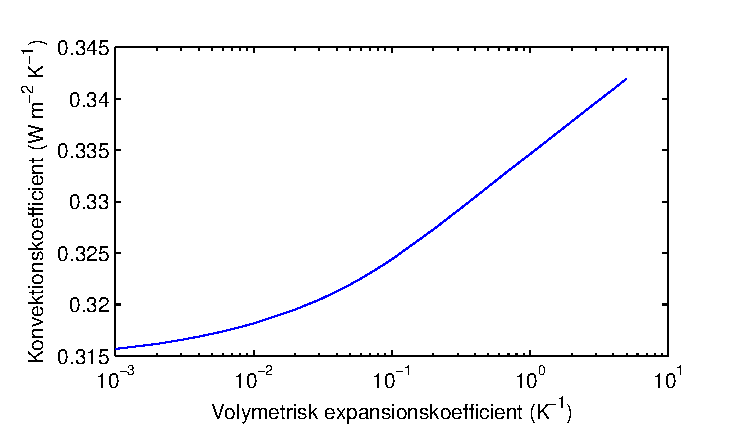
\includegraphics[scale=0.5]{images/convecbeta.eps}
}

\caption{\label{fig:konv_param}Stabilitets\-beräkningar av konvektions\-koefficienten h mot några
parametrar och natur\-konstanter i finita element\-simuleringen av Navier-Stokes ekvationer.
Inomhus\-temperaturen är satt konstant till $\unit[20]{^\circ C}$ med en vägg vars U-värde är
$\unit[1,19]{ W~m^{-2}~K^{-1}}$. Detta skall motsvara söder\-väggen på fastigheten som detta arbete behandlar.}

\end{figure}

% RESULTAT                                                                                                                                    
I figur~\ref{fig:h_reftemp} har beteendet hos metoden som bygger på finita elementmetoden studerats vid variation på några essentiella storheter i modellen.
Först har penaltyparametern varierats i figur~\ref{fig:h_penalty} och här kan det ses att modellens beteende inte förändras nämnvärt
beroende på val av parameter när denna närmar sig storleksordningen $\lambda = 10^7$. Det linjära förhållandet mellan
konvektionskoefficienten och temperaturdifferensen är intressant men saknar stöd i litteraturen då den rimligtvis borde vara
konstant eller nästan konstant. Slutligen varieras den volymetriska expansionskoefficienten
i figur~\ref{fig:h_volexp}. Det är denna storhet
som gör att luften stiger när den blir varm och det är av denna anledning fenomenet fri konvektion uppstår. Konvektionskoefficienten
ser ut att öka mer än logaritmiskt men däremot inte så snabbt. Anledningen till att penaltyparametern varierades var för
att studera hur stor den skulle behöva bli innan konvektionen började få samma energitransporterande egenskaper
som den förväntats ha. Som kan ses så kommer inte modellen ens i närheten av förväntat värde, inte ens då volymetrisk expansionskoefficient ett mycket högt värde.

Slutligen kan vi bara konstatera att det inte gick att använda denna metod för att studera konvektionsparametern $h$. Litteraturen
som ligger till grund för detta har använt sig av Streamline-Upwind/Petrov-Galerkin (SUPG)\cite{heinrich88}\cite{roy05}. Ovanstående metod är dock
Standard Galerkin med linjära triangulära element. Det är känt att Standard Galerkin kan leda till korsvindsproblem och lösningar som inte är
exakta och stabila\cite{segal2011}.
En misstanke är att det är detta problem vi ser även om detta inte verifieras genom att studera hastighetsfältet. Andra
möjliga orsaker kan vara randvillkor, för liten vald definitionsmängd eller något fel i den matematiska beskrivningen alternativt
vid implementeringen i Matlab.

\section{Datorsimulering av ofrivillig ventilation}

Ett hus är i praktiken omöjligt att göra helt tätt. Då vinden ligger på
får man därför ett drag genom huset, en ofrivillig ventilation. Då vinden
sällan är lika varm som inomhusluften leder detta till en energiförlust.
Den har beräknats med hjälp av programvaran Comsol. Problemets geometri har
setts upp enligt figur~ \ref{fig:windmethod:tri}. Bredvid fastigheten på Walleriusgatan ligger en annan byggnad och problemet med vind från de olika hållen blir symmetriskt. Blåser det från norr illustreras den för projektet aktuella fastigheten till höger i bild, och blåser det från söder påverkas den som den till vänster.

Från vänstra kanten så har luften blåst in med en konstant vindhastiget som varieras mellan olika
experiment. På andra sidan av fastigheterna har det satt ett konstant lufttryck som motsvarar en
atmosfärs tryck. På randerna som ligger mot mark eller mot hus är vindhastigheten satt till noll.
Slutligen utför ej luftmassan ovanför definitionsmängden någon kraft på luften som ligger längs den
övre randen.

\begin{figure}
\centering
\includegraphics[width=127mm,height=76mm]{images/triinfiltration.eps}
\caption{Triangulering samt definitionsmängd uppsatt för problemet.}\label{fig:windmethod:tri}
\end{figure}

Trycket inne i fastigheterna har sedan beräknats genom att luftläckaget antagits homogent utspritt över fastigheternas
väggar och att inget luft läckt genom taket. Därefter har Darcys lag satts upp med antagande om jämvikt så att lika mycket
luft som flödar in även kommer ut. Då både trycket inomhus och på ränderna är kända kan läckaget beräknas med Darcys lag
eller med någon annan exponent, se avsnitt~\ref{sec:darcy}. Här är antagandet gjort att huset läcker mycket och har $C(50)^{0,60} = 1,2$. \emph{\color{red} Vad menas här? Vad kom C ifrån? och siffrorna?} Dock kommer även exponenten ha betydelse för läckaget.\cite{sasic}

